\documentclass[12pt]{article}%
\usepackage{tikz}
\usepackage{latexsym, amsmath,amsfonts,amssymb}
\usepackage{xcolor}
\usepackage[margin=.75in]{geometry}
\linespread{1.1}
\pagestyle{empty}
\begin{document}

\begin{center}
\Large{\textbf{Japanese Line Functions (Amidakuji) are 1-1}}
\end{center}
Amidakuji are examples of permuations groups so they
must be 1-1 functions but that explanation isn't appropriate 
for your high school math class. First, an Amidakuji is a 
function because the well defined rules of movement ensure 
that just one movement is possible: down, right, or left. To 
explain why it's 1-1 I'm going to talk about points in each 
path by which I mean the points where a path changes 
direction. Points occur when horizontal and vertical line 
segments intersect.
\begin{figure}[h!]
\begin{minipage}{.6\textwidth}
\begin{center}
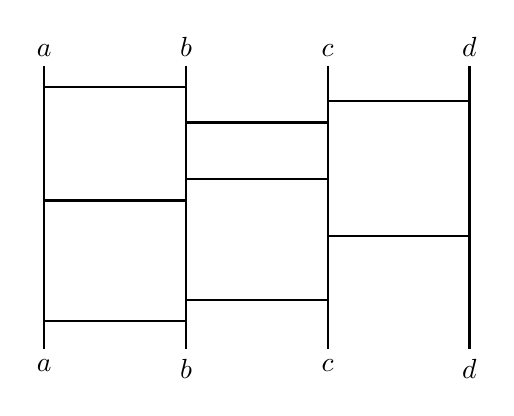
\begin{tikzpicture}[scale=.9]
\foreach \x in {0, ...,3}{
\draw[thick] (2*\x+1,4)--(2*\x+1,0);
}
\coordinate [label=above:$a$] (a1) at (1,4);
\coordinate [label=below:$a$] (a2) at (1,0);
\coordinate [label=above:$b$] (b1) at (3,4);
\coordinate [label=below:$b$] (b2) at (3,0);
\coordinate [label=above:$c$] (c1) at (5,4);
\coordinate [label=below:$c$] (c2) at (5,0);
\coordinate [label=above:$d$] (d1) at (7,4);
\coordinate [label=below:$d$] (d2) at (7,0);
\draw[thick] (1,3.7)--(3,3.7);
\draw[thick] (1,2.1)--(3,2.1);
\draw[thick] (1,.4)--(3,.4);
\draw[thick] (3,3.2)--(5,3.2);
\draw[thick] (3,2.4)--(5,2.4);
\draw[thick] (3,.7)--(5,.7);
\draw[thick] (5,3.5)--(7,3.5);
\draw[thick] (5,1.6)--(7,1.6);
\end{tikzpicture}
\end{center}
\end{minipage}
\begin{minipage}{.4\textwidth}
\begin{center}
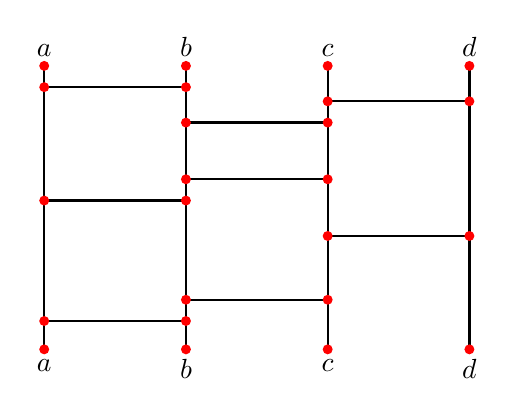
\begin{tikzpicture}[scale=.9]
\foreach \x in {0, ...,3}{
\draw[thick] (2*\x+1,4)--(2*\x+1,0);
}
\coordinate [label=above:$a$] (a1) at (1,4);
\coordinate [label=below:$a$] (a2) at (1,0);
\coordinate [label=above:$b$] (b1) at (3,4);
\coordinate [label=below:$b$] (b2) at (3,0);
\coordinate [label=above:$c$] (c1) at (5,4);
\coordinate [label=below:$c$] (c2) at (5,0);
\coordinate [label=above:$d$] (d1) at (7,4);
\coordinate [label=below:$d$] (d2) at (7,0);
\draw[thick] (1,3.7)--(3,3.7);
\draw[thick] (1,2.1)--(3,2.1);
\draw[thick] (1,.4)--(3,.4);
\draw[thick] (3,3.2)--(5,3.2);
\draw[thick] (3,2.4)--(5,2.4);
\draw[thick] (3,.7)--(5,.7);
\draw[thick] (5,3.5)--(7,3.5);
\draw[thick] (5,1.6)--(7,1.6);
\foreach\x in {1,3,5,7}{
\fill[red] (\x cm,4cm) circle (2pt);
\fill[red] (\x cm,0cm) circle (2pt);
}
\fill[red] (1cm,3.7cm) circle (2pt);
\fill[red] (1cm,2.1cm) circle (2pt);
\fill[red] (1cm,.4cm) circle (2pt);
\fill[red] (3cm,3.7cm) circle (2pt);
\fill[red] (3cm,3.2cm) circle (2pt);
\fill[red] (3cm,2.4cm) circle (2pt);
\fill[red] (3cm,2.1cm) circle (2pt);
\fill[red] (3cm,.7cm) circle (2pt);
\fill[red] (3cm,.4cm) circle (2pt);
\fill[red] (5cm,3.5cm) circle (2pt);
\fill[red] (5cm,3.2cm) circle (2pt);
\fill[red] (5cm,2.4cm) circle (2pt);
\fill[red] (5cm,1.6cm) circle (2pt);
\fill[red] (5cm,.7cm) circle (2pt);
\fill[red] (7cm,3.5cm) circle (2pt);
\fill[red] (7cm,1.6cm) circle (2pt);
\end{tikzpicture}
\end{center}
\end{minipage}
\caption{If two different paths intersect it will be at a 
red point.}
\end{figure}

\noindent\textbf{Theorem:} Every Amidakuji (Japanese 
line function) is 1-1.\\
\textbf{Proof:} For every Japanese line function we can 
describe the path from one letter at the top to the letter it 
goes to on the bottom using a sequence of the letters D 
(down), L (left), and R (right). From the way Amidakuji
are constructed every sequence begins with D and ends 
with a D. Now suppose, by way of contradiction, there's 
an Amidakuji which is not 1-1; then there exist 2 sequences
of moves that start from different letters at the
top and end at the same letter at the bottom. Since the
two paths have a common ending point, let $p$ be
the first point that the 2 sequences have in common 
after which the 2 sequences are identical. The question
is what were the moves just before the 2 paths  got to $p$?\\
\textbf{Case 1:} \underline{Both paths got to $p$ by 
moving direction D.} (DD) By the definition of $p$, one point 
is higher than the other; that is we have on the same 
vertical line points $p$, $y_1$ and $y_2$ where $y_2$ is 
above $y_1$ which is above $p$. Moving direction D from 
$y_2$ will stop at some point (which, at the latest, is 
$y_1$) and then it moves L or R, hence doesn't end at $p$,
a contradiction.\\
\textbf{Case 2:} \underline{Both paths got to $p$ by 
moving direction L or R. } (LL, RR) A horizontal line 
can't span more than 2 vertical lines so both paths started 
at the same point $s$ and moved L (or R) to get to $p$. 
That's a contradiction because $p$ is the first point in 
common after which the paths become identical.\\
\textbf{Case 3:} \underline{One path got to $p$
moving direction L, the other by moving
direction R.} (LR, RL) This implies there is a horizontal
line segment spanning more than 2 consecutive vertical
lines, contradicting the way Amidakuji are created.\\
\textbf{Case 4:} \underline{One path got to $p$ moving 
direction D, the other by moving direction R (or L).} (DR, DL, 
LD, RD) After moving direction D to get to $p$ the sequence
would have to continue with L (or R) while the other 
sequence has to move direction D. Therefore, the next 
point on the sequences is different, contradicting 
the definition of $p$.

All cases result in a contradiction; it follows that every 
Amidakuji is a 1-1 function.
\end{document}